\documentclass[12pt]{article}
\usepackage[margin=0.9in,headheight=16pt]{geometry}
\usepackage[T1]{fontenc}
\usepackage{lmodern}
\usepackage{graphicx}
\graphicspath{{../../figures/}{../figures/}{figures/}}
\usepackage{array}
\usepackage{booktabs}
\usepackage{longtable}
\usepackage{tabularx}
\usepackage{float}
\usepackage{caption}
\usepackage{amsmath}
\usepackage{amssymb}
\usepackage{tikz}
\usetikzlibrary{arrows.meta,positioning,shapes.geometric}
\usepackage{enumitem}
\usepackage{hyperref}
\usepackage{xcolor}
\usepackage{etoolbox}
\usepackage{fancyhdr}
\usepackage{titlesec}
\usepackage{setspace}

\definecolor{psidblue}{HTML}{1E3A5F}
\definecolor{psidink}{HTML}{1F2937}
\definecolor{psidmuted}{HTML}{4B5563}
\definecolor{psidline}{HTML}{D1D5DB}
\definecolor{psidpanel}{HTML}{F7FAFC}
\definecolor{psidaccent}{HTML}{E8F1FB}
\definecolor{psidgold}{HTML}{A16207}

\hypersetup{
  colorlinks=true,
  linkcolor=psidblue,
  urlcolor=psidblue,
  citecolor=psidblue,
  pdftitle={PSID Client Report},
  pdfauthor={GitHub Copilot}
}

\makeatletter
\g@addto@macro\UrlBreaks{\do\_\do\/\do\-}
\makeatother

\captionsetup{
  font=small,
  labelfont={bf,sf,color=psidblue},
  justification=raggedright,
  singlelinecheck=false
}
\captionsetup[table]{position=top}

\setlength{\parindent}{0pt}
\setlength{\parskip}{5pt}
\setlength{\tabcolsep}{3.5pt}
\setlength{\LTleft}{0pt}
\setlength{\LTright}{0pt}
\renewcommand{\arraystretch}{1.14}
\setlist[itemize]{leftmargin=1.5em, itemsep=0.2em, topsep=0.3em}
\setlist[enumerate]{leftmargin=1.6em, itemsep=0.25em, topsep=0.3em}
\setstretch{1.08}
\emergencystretch=1.5em

\newcolumntype{L}[1]{>{\raggedright\arraybackslash\hspace{0pt}}p{#1}}
\newcolumntype{C}[1]{>{\centering\arraybackslash}p{#1}}
\newcolumntype{R}[1]{>{\raggedleft\arraybackslash}p{#1}}
\newcolumntype{Y}{>{\raggedright\arraybackslash\hspace{0pt}}X}

\newcommand{\reportseries}{PSID Crisis Module Client Series}
\newcommand{\reporttitle}{Client Report}
\newcommand{\reportsubtitle}{PSID Crisis Module}
\newcommand{\reportclient}{Client Deliverable}
\newcommand{\reportversion}{April 2026}
\newcommand{\reportstatus}{Prepared for client review}
\newcommand{\reportabstract}{}
\newcommand{\reportkeywords}{}
\newcommand{\reportdoi}{\url{https://github.com/namo507/Team-PSID}}
\newcommand{\varname}[1]{\nolinkurl{#1}}
\newcommand{\filepath}[1]{\nolinkurl{#1}}

\pagestyle{fancy}
\fancyhf{}
\fancyhead[L]{\sffamily\footnotesize \reporttitle}
\fancyhead[R]{\sffamily\footnotesize \thepage}
\fancyfoot[L]{\sffamily\footnotesize \reportclient}
\fancyfoot[R]{\sffamily\footnotesize Team-PSID}

\fancypagestyle{plain}{
  \fancyhf{}
  \fancyhead[L]{\sffamily\footnotesize \reporttitle}
  \fancyhead[R]{\sffamily\footnotesize \thepage}
  \fancyfoot[L]{\sffamily\footnotesize \reportclient}
  \fancyfoot[R]{\sffamily\footnotesize Team-PSID}
}

\titleformat{\section}{\Large\bfseries\sffamily\color{psidblue}}{\thesection}{0.75em}{}
\titleformat{\subsection}{\large\bfseries\sffamily\color{psidink}}{\thesubsection}{0.65em}{}
\titleformat{\subsubsection}{\normalsize\bfseries\sffamily\color{psidink}}{\thesubsubsection}{0.5em}{}

\newsavebox{\psidboxbox}
\newenvironment{psidbox}[1]{%
  \par\medskip
  \begin{center}
  \setlength{\fboxsep}{12pt}%
  \begin{lrbox}{\psidboxbox}
  \begin{minipage}{0.94\linewidth}
  {\sffamily\bfseries\color{psidblue}#1}\par\medskip
}{%
  \end{minipage}
  \end{lrbox}
  \fcolorbox{psidline}{psidpanel}{\usebox{\psidboxbox}}
  \end{center}
  \par\medskip
}

\newcommand{\makecover}{%
  \pagenumbering{arabic}
  \thispagestyle{plain}
  {\sffamily\footnotesize\color{psidmuted}\reportseries\hfill \reportclient\par}
  \vspace{0.35cm}
  {\sffamily\bfseries\fontsize{22}{26}\selectfont \reporttitle\par}
  \vspace{0.15cm}
  {\sffamily\Large\color{psidmuted} \reportsubtitle\par}
  \vspace{0.3cm}
  {\footnotesize\color{psidmuted}\reportstatus\quad|\quad Updated: \reportversion\quad|\quad \reportdoi\par}
  \vspace{0.35cm}
  \begin{psidbox}{Abstract}
  \reportabstract
  \end{psidbox}
  \ifstrempty{\reportkeywords}{}{%
    {\sffamily\small\textbf{Keywords:} \reportkeywords\par}
    \vspace{0.2cm}
  }
  {\color{psidline}\rule{\textwidth}{0.9pt}}\par
  \vspace{0.45cm}
}

\newcommand{\psidfigure}[3][0.92]{%
  \begin{figure}[H]
  \centering
  \fcolorbox{psidline}{white}{\includegraphics[width=#1\linewidth]{#2}}
  \caption{#3}
  \end{figure}
}

\tikzset{
  flowstep/.style={
    rectangle,
    rounded corners=6pt,
    draw=psidblue,
    fill=psidpanel,
    very thick,
    align=center,
    text width=3.6cm,
    minimum height=1cm,
    font=\sffamily\small
  },
  flowwide/.style={flowstep, text width=4.4cm},
  flowresult/.style={flowstep, draw=psidgold!85!black, fill=psidaccent},
  flowarrow/.style={-{Stealth[length=3mm]}, very thick, draw=psidblue}
}

\renewcommand{\reporttitle}{Client 2: Deployable Questionnaire}
\renewcommand{\reportsubtitle}{Administration-ready questionnaire guide with universe rules, timing, and row-level rationale}
\renewcommand{\reportclient}{Operational Deliverable}
\renewcommand{\reportabstract}{This operational report converts the scored PSID crisis-module output into a field-ready questionnaire with routing rules, timing estimates, and row-level rationale. It explains how the 28-row scored module becomes a 26-question deployable instrument, how respondent answers activate only one relevant crisis block, and how the final field package preserves analytic traceability while reducing burden.}
\renewcommand{\reportkeywords}{deployable questionnaire | crisis routing | respondent burden | PSID module | field administration}

\begin{document}

\makecover

\section{Purpose}

This report is the PDF-ready version of the deployable questionnaire package. It translates the final scored question bank into a practical administration guide with live question tables, universe rules, timing estimates, and the ranking logic behind selection.

\begin{psidbox}{Deployable scope}
This deployable version begins from the same 28-row scored module used in the technical review package. It excludes \varname{SPC_AGE_YEARS} $(0.35$ minutes$)$ and \varname{SPC_DESCRIBE_SEX_GENDER} $(0.817$ minutes$)$, which remain in the master review file for traceability but are removed from routine field administration. The result is a 26-question instrument with an estimated paper length of $29.98 - 0.35 - 0.817 = 28.82$ minutes.
\end{psidbox}

\section{Deployable Snapshot}

\begin{table}[H]
\centering
\small
\begin{tabularx}{\textwidth}{L{0.22\textwidth} R{0.10\textwidth} Y Y}
\toprule
Metric & Value & Calculation / rule & Why it is used and the assumption behind it \\
\midrule
Deployable questions & 26 & $28 - 2 = 26$ after removing the selected demographic-only rows & Defines the paper instrument that can be handed to field staff. \\
Estimated deployable minutes & 28.82 & $29.98 - 0.35 - 0.817 = 28.813 \approx 28.82$ & Upper-bound paper length if the full deployable document is read end to end. \\
All-respondent Generic questions & 3 & Count of rows asked before any routing logic is applied & Portable screening core; assumes every respondent should receive the same baseline crisis probe. \\
Pandemic or public-health questions & 5 & Count of rows in the pandemic block & Activated only when respondent answers or interview context indicate a pandemic/public-health event. \\
Shutdown or financial-disruption questions & 4 & Count of rows in the shutdown/financial-disruption block & Activated only when the crisis is economic or shutdown driven. \\
Disaster, displacement, or direct-exposure questions & 14 & Count of rows in the disaster/displacement block & Largest block because direct-exposure content carries the richest disaster signal in the source bank. \\
\bottomrule
\end{tabularx}
\caption{Deployable instrument summary after removing demographic-only rows.}
\end{table}

\section{Figures and Visual Diagnostics}

\psidfigure{fig_time_budget.png}{Time-budget allocation across the selected scored module.}
\psidfigure{fig_top_ranked_questions.png}{Top-ranked items retained in the refreshed package.}
\psidfigure{fig_toggle_comparison.png}{Binary Generic versus Specific split used to route administration.}

\section{Deployable Workflow Pipeline}

\begin{figure}[H]
\centering
\resizebox{0.88\textwidth}{!}{%
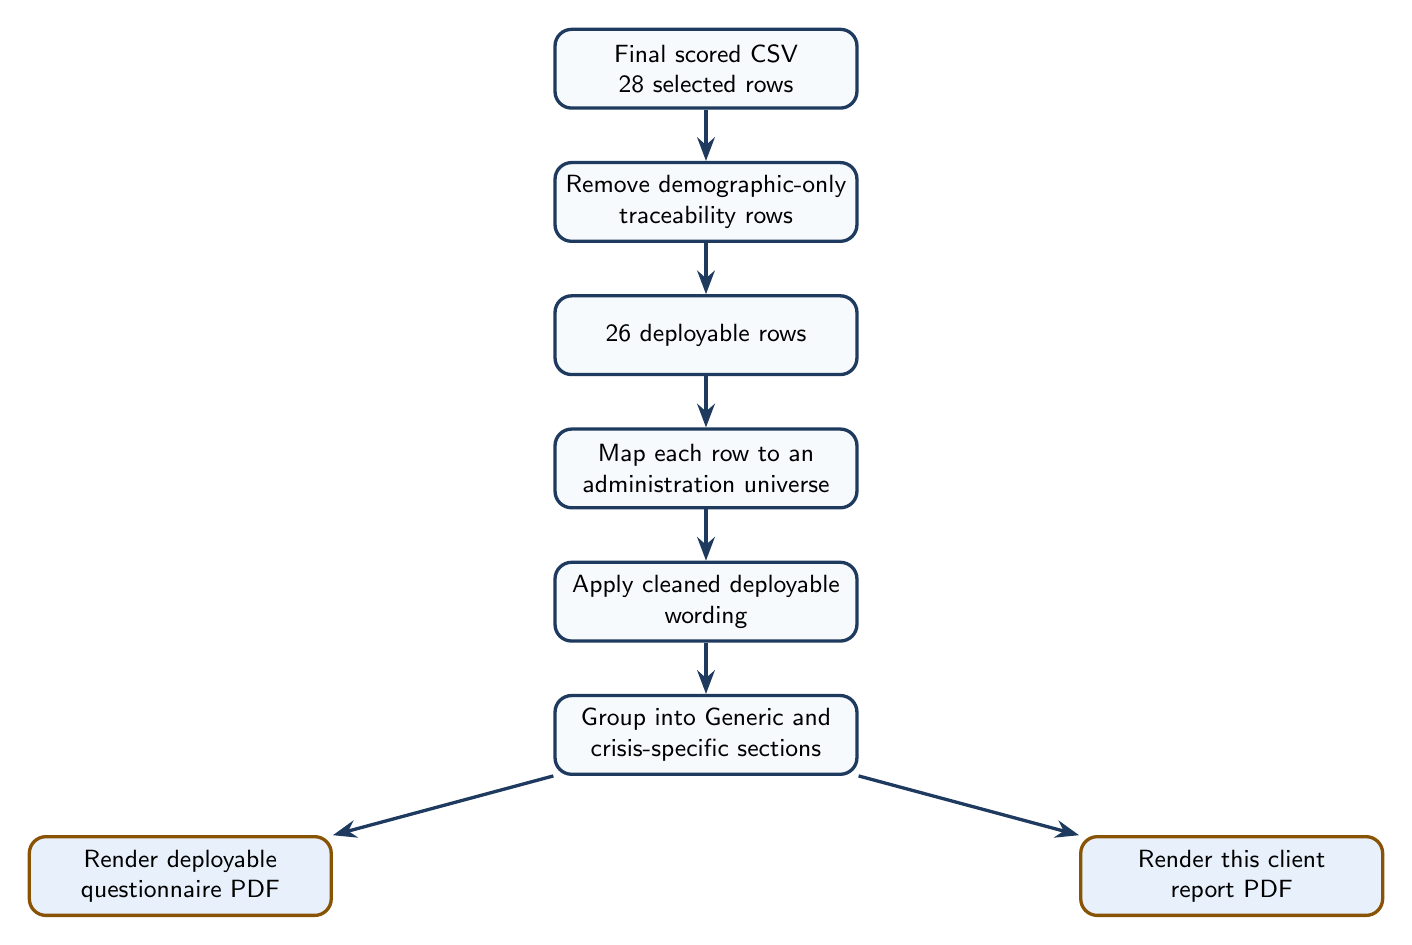
\begin{tikzpicture}[node distance=0.65cm]
\node[flowstep] (a) {Final scored CSV\\28 selected rows};
\node[flowstep, below=of a] (b) {Remove demographic-only\\traceability rows};
\node[flowstep, below=of b] (c) {26 deployable rows};
\node[flowstep, below=of c] (d) {Map each row to an\\administration universe};
\node[flowstep, below=of d] (e) {Apply cleaned deployable\\wording};
\node[flowstep, below=of e] (f) {Group into Generic and\\crisis-specific sections};
\node[flowresult, below left=0.75cm and 2.8cm of f] (g) {Render deployable\\questionnaire PDF};
\node[flowresult, below right=0.75cm and 2.8cm of f] (h) {Render this client\\report PDF};
\draw[flowarrow] (a) -- (b);
\draw[flowarrow] (b) -- (c);
\draw[flowarrow] (c) -- (d);
\draw[flowarrow] (d) -- (e);
\draw[flowarrow] (e) -- (f);
\draw[flowarrow] (f) -- (g);
\draw[flowarrow] (f) -- (h);
\end{tikzpicture}
}
\caption{Operational path from the scored module to the deployable questionnaire package.}
\end{figure}

\section{Why 28 Scored Rows Become 26 Asked Questions}

\begin{table}[H]
\centering
\footnotesize
\begin{tabularx}{\textwidth}{L{0.22\textwidth} R{0.08\textwidth} R{0.10\textwidth} Y Y}
\toprule
Stage & Rows & Minutes & Calculation / rule & Operational meaning \\
\midrule
Scored module & 28 & 29.98 & Count and summed minutes for rows with \texttt{selected\_for\_module = True} & Full analytic shortlist retained for auditability and review. \\
Selected demographic traceability rows & 2 & 1.17 & \varname{SPC_AGE_YEARS} $(0.35)$ + \varname{SPC_DESCRIBE_SEX_GENDER} $(0.817)$ & Context variables retained in the master file but not asked by default in the crisis instrument. \\
Deployable paper instrument & 26 & 28.82 & $28 - 2 = 26$ and $29.98 - 1.167 = 28.813 \approx 28.82$ & Clean field-ready questionnaire containing only direct crisis items plus the universal Generic screen. \\
\bottomrule
\end{tabularx}
\caption{The 28-to-26 change is a deployment-stage subtraction, not a change in the scoring model.}
\end{table}

\section{Optimization Change From Scored Review to Live Administration}

\begin{table}[H]
\centering
\small
\begin{tabularx}{\textwidth}{L{0.20\textwidth} Y Y Y}
\toprule
Dimension & Legacy architecture view & Current deployable view & Operational effect \\
\midrule
Category structure & Legacy architecture used 7 Generic Core rows, 1 Financial Crisis row, and 20 Pandemic / Disaster rows in the 28-row architecture & Current deployment asks 3 universal Generic rows first, then one routed crisis-specific block from a 23-row Specific bank & The universal screen is shorter and the field instrument is easier to explain. \\
Financial items & Financial questions were visible as their own toggle label & Financial questions now compete inside Specific under the same redundancy and portability logic as other crisis items & Duplicate earnings or aid variants no longer dominate the field package. \\
Deployment target & The scored shortlist and the field-facing package were closer together & The 28-row scored module remains the audit record, while the 26-row deployable file is the asked instrument & Separates internal traceability from respondent burden. \\
Optimization levers & Ranking plus legacy toggle structure & Ranking plus portability bonus, redundancy control, construct coverage, documented wording replacements, and respondent-answer routing & Produces a more defensible always-on instrument. \\
\bottomrule
\end{tabularx}
\caption{How the deployable questionnaire was optimized relative to the older architecture view.}
\end{table}

\section{Administration Rules}

\subsection{Administration sequence}

\begin{enumerate}
\item Ask the three all-respondent Generic items.
\item Identify the active crisis context.
\item Activate one crisis-specific section based on that context and on the respondent's Generic-core answers.
\item Skip all sections that do not match the active crisis.
\end{enumerate}

\subsection{Respondent-answer refinement and live path lengths}

\begin{table}[H]
\centering
\small
\begin{tabularx}{\textwidth}{L{0.22\textwidth} R{0.08\textwidth} R{0.10\textwidth} Y Y}
\toprule
Live path & Rows asked & Minutes & Calculation / rule & Why it is used and the assumption behind it \\
\midrule
Pandemic path & 8 & 4.32 & $3$ Generic $+ 5$ pandemic rows and $1.40 + 2.92 = 4.32$ minutes & Used when answers or interview context indicate a pandemic/public-health event; assumes only the relevant block is activated. \\
Shutdown path & 7 & 5.60 & $3$ Generic $+ 4$ shutdown rows and $1.40 + 4.20 = 5.60$ minutes & Used for acute financial disruption or shutdown crises; assumes one dominant economic-disruption context. \\
Disaster path & 17 & 21.70 & $3$ Generic $+ 14$ disaster rows and $1.40 + 20.30 = 21.70$ minutes & Used for displacement, trauma, or direct exposure events; longest path because the disaster bank carries the deepest direct-impact content. \\
Full paper instrument & 26 & 28.82 & Sum of all deployable rows listed in this document & Upper bound shown for documentation; not the default live path for a single respondent. \\
\bottomrule
\end{tabularx}
\caption{Respondent answers refine the effective interview length by activating one relevant crisis block.}
\end{table}

\subsection{Universe summary}

\begin{table}[H]
\centering
\begin{tabularx}{\textwidth}{L{0.34\textwidth} R{0.08\textwidth} R{0.10\textwidth} R{0.10\textwidth} R{0.10\textwidth}}
\toprule
Universe block & Rows & Minutes & Average $R_i$ & Average $P_i$ \\
\midrule
All respondents & 3 & 1.40 & 5.334 & 7.125 \\
Pandemic or public-health emergency & 5 & 2.92 & 3.364 & 4.393 \\
Shutdown, recession, or acute financial disruption & 4 & 4.20 & 3.424 & 4.509 \\
Disaster, displacement, or direct exposure event & 14 & 20.30 & 2.617 & 2.768 \\
\bottomrule
\end{tabularx}
\caption{Universe blocks used to route live administration.}
\end{table}

\subsection{Source contribution to the deployable instrument}

\begin{table}[H]
\centering
\begin{tabularx}{0.64\textwidth}{L{0.34\textwidth} R{0.10\textwidth} R{0.10\textwidth}}
\toprule
Source & Rows & Minutes \\
\midrule
Hurricane Katrina 2007 & 14 & 20.30 \\
COVID-19 & 8 & 4.32 \\
Govt Shutdown Income & 3 & 2.33 \\
Govt Shutdown Crisis & 1 & 1.87 \\
\bottomrule
\end{tabularx}
\caption{Historical source contribution to the deployable questionnaire.}
\end{table}

\section{Formula Notes for Deployment}

The deployable questionnaire still comes from the same scoring logic as the full codebook.

\begin{psidbox}{Operational formulae}
\begin{align*}
\text{minutes} &= \frac{\text{word\_count} \times 7}{60} \\
R_i &= \frac{U_i}{B_i} \\
P_i &= \frac{\text{augmented\_utility}}{B_i \times (1 + 0.65 \times \text{redundancy\_scaled})}
\end{align*}

\begin{itemize}
\item $R_i$ explains why a question is strong relative to burden.
\item $P_i$ helps decide which similar questions survive the time-budget cut.
\item Minutes is the operational field used for questionnaire assembly.
\end{itemize}
\end{psidbox}

\begin{table}[H]
\centering
\small
\begin{tabularx}{\textwidth}{L{0.18\textwidth} Y Y Y}
\toprule
Quantity & Calculation & Why it is used & Assumption \\
\midrule
minutes & $(\text{word\_count} \times 7)/60$ & Converts wording length into an operational time field for routing and budget control & Oral administration averages about 7 seconds per word. \\
$R_i$ & $U_i / B_i$ & Explains why a row is strong relative to its burden & Efficient questions should deliver more crisis signal than the time they consume. \\
$P_i$ & $\text{augmented\_utility} / [B_i \times (1 + 0.65\,\text{redundancy\_scaled})]$ & Breaks ties among similarly efficient rows by rewarding distinctiveness and portability & A short field instrument should prefer distinct rows over repeated variants. \\
Deployable rows & Selected scored rows minus demographic-only traceability rows & Converts the audit package into the field instrument & Demographic context is not part of the default asked path. \\
Live path length & Generic-core minutes plus one active crisis block & Translates the paper instrument into respondent-specific burden & Exactly one specific block is active for the standard administration path. \\
\bottomrule
\end{tabularx}
\caption{How the main deployable quantities are derived and interpreted.}
\end{table}

\section{Worked Example for a Deployable Generic Item}

Example question: \varname{GEN_LOSE_EARNINGS_PANDEMIC}

\begin{table}[H]
\centering
\begin{tabularx}{\textwidth}{L{0.18\textwidth} R{0.12\textwidth} Y Y}
\toprule
Field & Value & Calculation & Why it is used / assumption \\
\midrule
Question text & Did you lose earnings because of the pandemic? & Clean deployable wording retained in the universal screen & This item is portable enough to ask before any crisis-specific routing begins. \\
$U_i$ & 3.400 & $0.80 + 0.80 + 0.90 + 0.90$ & Utility aggregates matched crisis-signal weights; assumes the tagged keywords capture the substance of the item. \\
$B_i$ & 0.600 & $\max(0.10 \times 6 + 0.20 \times 0.0, 0.1)$ & Burden penalizes wording cost; assumes the fixed burden constants remain the operational design choice. \\
$R_i$ & 5.667 & $3.40 / 0.60$ & Shows why the row is analytically strong relative to burden. \\
$P_i$ & 7.860 & Value computed after rarity, construct, portability, and redundancy scaling & Keeps the item ahead of lower-value or more repetitive alternatives. \\
minutes & 0.70 & $(6 \times 7) / 60$ & Feeds the routing and time-budget calculations; assumes 7 seconds per word in oral administration. \\
Administration block & All respondents & Asked before any crisis-specific skip logic & Assumes every respondent should receive a common crisis-baseline screen. \\
\bottomrule
\end{tabularx}
\caption{Worked example showing how one Generic item remains short, portable, and analytically strong.}
\end{table}

\section{All-Respondent Generic Core}

These questions create a portable core that can be asked before event-specific routing.

\begin{table}[H]
\centering
\scriptsize
\setlength{\tabcolsep}{3pt}
\begin{tabularx}{\textwidth}{@{}L{0.17\textwidth} L{0.13\textwidth} L{0.31\textwidth} R{0.07\textwidth} R{0.07\textwidth} R{0.08\textwidth}@{}}
\toprule
Variable & Source & Question & $R_i$ & $P_i$ & Minutes \\
\midrule
\varname{GEN_EXPERIENCED_FINANCIAL_DIFFICULTIES_C} & COVID-19 & Have you experienced any financial difficulties because of the crisis? & 5.667 & 7.187 & 0.35 \\
\varname{GEN_LOSE_EARNINGS_PANDEMIC} & COVID-19 & Did you lose earnings because of the pandemic? & 5.667 & 7.860 & 0.70 \\
\varname{GEN_RECEIVE_STIMULUS_PAYMENT_OTHER} & COVID-19 & Did you receive a stimulus payment or other emergency government support? & 4.667 & 6.328 & 0.35 \\
\bottomrule
\end{tabularx}
\caption{All-respondent Generic core.}
\end{table}

\section{Pandemic or Public-Health Emergency Block}

Ask this section when the active crisis is a pandemic or other public-health emergency.

\begin{table}[H]
\centering
\scriptsize
\setlength{\tabcolsep}{3pt}
\begin{tabularx}{\textwidth}{@{}L{0.17\textwidth} L{0.13\textwidth} L{0.31\textwidth} R{0.07\textwidth} R{0.07\textwidth} R{0.08\textwidth}@{}}
\toprule
Variable & Source & Question & $R_i$ & $P_i$ & Minutes \\
\midrule
\varname{SPC_WORK_ENTIRELY_HOME_DURING} & COVID-19 & Did you work entirely from home during the crisis? & 3.500 & 3.957 & 0.47 \\
\varname{SPC_WORKING_JOB_CONSIDERED_ESSENTIAL} & COVID-19 & Were you working in a job that was considered essential during the crisis? & 4.000 & 5.223 & 1.05 \\
\varname{SPC_RECEIVE_PAYCHECK_PROTECTION_OTHER} & COVID-19 & Did you receive paycheck protection or other emergency business support? & 3.500 & 5.212 & 0.23 \\
\varname{SPC_RECEIVE_STIMULUS_PAYMENT_OTHER} & COVID-19 & Did you receive a stimulus payment or other emergency government support? & 3.500 & 4.466 & 0.23 \\
\varname{SPC_LAID_OFF_FURLOUGHED_PANDEMIC} & COVID-19 & Were you laid off or furloughed because of the pandemic? & 2.318 & 3.106 & 0.93 \\
\bottomrule
\end{tabularx}
\caption{Pandemic or public-health emergency block.}
\end{table}

\section{Shutdown, Recession, or Acute Financial Disruption Block}

Ask this section when the active crisis is a shutdown, recession, or acute financial disruption.

\begin{table}[H]
\centering
\scriptsize
\setlength{\tabcolsep}{3pt}
\begin{tabularx}{\textwidth}{@{}L{0.17\textwidth} L{0.13\textwidth} L{0.31\textwidth} R{0.07\textwidth} R{0.07\textwidth} R{0.08\textwidth}@{}}
\toprule
Variable & Source & Question & $R_i$ & $P_i$ & Minutes \\
\midrule
\varname{SPC_STOPPED_WORK_CRISIS} & Govt Shutdown Income & Have you stopped this work because of the crisis? & 3.500 & 4.134 & 0.47 \\
\varname{SPC_WAGES_SALARY_PAYMENTS_JOB} & Govt Shutdown Income & Were there any wages or salary payments from this job during the crisis period? & 2.727 & 4.134 & 1.17 \\
\varname{SPC_HOUSEHOLD_MANAGE_FINANCIAL_DIFFICULT} & Govt Shutdown Crisis & How did your household manage financial difficulties caused by the shutdown or crisis? & 3.719 & 4.592 & 1.87 \\
\varname{SPC_STOPPED_WORKING_BUSINESS_CRISIS} & Govt Shutdown Income & Have you stopped working at this business because of the crisis? & 3.750 & 5.177 & 0.70 \\
\bottomrule
\end{tabularx}
\caption{Shutdown, recession, or acute financial disruption block.}
\end{table}

\section{Disaster, Displacement, or Direct Exposure Block}

Ask this section when the active crisis is a disaster, displacement, or direct exposure event.

\begin{table}[H]
\centering
\scriptsize
\setlength{\tabcolsep}{3pt}
\begin{tabularx}{\textwidth}{@{}L{0.17\textwidth} L{0.13\textwidth} L{0.31\textwidth} R{0.07\textwidth} R{0.07\textwidth} R{0.08\textwidth}@{}}
\toprule
Variable & Source & Question & $R_i$ & $P_i$ & Minutes \\
\midrule
\varname{SPC_HOME_DAMAGED_DESTROYED_DISASTER} & Hurricane Katrina 2007 & Was your home damaged or destroyed by the disaster? & 2.650 & 2.266 & 1.17 \\
\varname{SPC_BUSINESS_DAMAGED_DESTROYED_DISASTER} & Hurricane Katrina 2007 & Was your business damaged or destroyed by the disaster? & 3.300 & 2.962 & 1.17 \\
\varname{SPC_ANYONE_IMMEDIATE_FAMILY_KILLED} & Hurricane Katrina 2007 & Was anyone in your immediate family killed as a result of the disaster? & 2.115 & 2.060 & 1.52 \\
\varname{SPC_EXPERIENCE_HURRICANE_FORCE_WINDS} & Hurricane Katrina 2007 & Did you experience hurricane force winds at your location during the disaster? & 2.077 & 2.106 & 1.52 \\
\varname{SPC_EXPERIENCE_MAJOR_FLOODING_HOME} & Hurricane Katrina 2007 & Did you experience major flooding in your home during the disaster? & 3.792 & 4.222 & 1.40 \\
\varname{SPC_PHYSICALLY_INJURED_WAY_AS} & Hurricane Katrina 2007 & Were you physically injured in any way as a result of the disaster? & 2.846 & 2.804 & 1.52 \\
\varname{SPC_SEVERE_DAMAGE_HOME_DURING} & Hurricane Katrina 2007 & How severe was the damage to your home during the disaster? & 2.769 & 3.169 & 1.52 \\
\bottomrule
\end{tabularx}
\caption{Disaster, displacement, or direct exposure block: housing, damage, and direct physical exposure items.}
\end{table}

\begin{table}[H]
\centering
\scriptsize
\setlength{\tabcolsep}{3pt}
\begin{tabularx}{\textwidth}{@{}L{0.17\textwidth} L{0.13\textwidth} L{0.31\textwidth} R{0.07\textwidth} R{0.07\textwidth} R{0.08\textwidth}@{}}
\toprule
Variable & Source & Question & $R_i$ & $P_i$ & Minutes \\
\midrule
\varname{SPC_AFRAID_DURING_DISASTER_MIGHT} & Hurricane Katrina 2007 & How afraid were you during the disaster that you might be seriously injured or killed? & 2.447 & 2.584 & 1.87 \\
\varname{SPC_DISASTER_OFTEN_DISTURBING_MEMORIES} & Hurricane Katrina 2007 & Since the disaster, how often have you had disturbing memories or images about what happened? & 1.825 & 1.588 & 2.10 \\
\varname{SPC_LONG_STAY_TEMPORARY_HOUSING} & Hurricane Katrina 2007 & How long did you stay in temporary housing after the disaster? & 2.455 & 3.090 & 1.28 \\
\varname{SPC_EVACUATE_HOME_DISASTER_HIT} & Hurricane Katrina 2007 & Did you evacuate from your home before the disaster hit? & 3.227 & 3.530 & 1.28 \\
\varname{SPC_DISASTER_CAUSE_LOSE_JOB} & Hurricane Katrina 2007 & Did the disaster cause you to lose your job? & 3.200 & 3.708 & 1.17 \\
\varname{SPC_DISPLACED_PLACE_LIVING_DISASTER} & Hurricane Katrina 2007 & Were you displaced from the place you were living because of the disaster? & 2.115 & 2.643 & 1.52 \\
\varname{SPC_RECEIVE_HELP_FEMA_FEDERAL} & Hurricane Katrina 2007 & Did you receive any help from FEMA Federal Emergency Management Agency? & 1.818 & 2.027 & 1.28 \\
\bottomrule
\end{tabularx}
\caption{Disaster, displacement, or direct exposure block: trauma, displacement, employment, and aid items.}
\end{table}

\section{Administration Notes}

\begin{itemize}
\item The deployable questionnaire intentionally keeps the three \texttt{Generic} questions first because they travel best across crisis contexts.
\item The deployable file excludes demographic-only rows even though those rows still appear in the master review sheet.
\item Respondent answers refine the live path length: most interviews ask the 3-item Generic core plus one specific block rather than all 26 deployable rows.
\item Some closely related support items appear in both the Generic and pandemic blocks because one version is meant for universal framing and the other is preserved as an event-specific probe.
\item The disaster block is the longest because the Katrina source bank contributes the richest direct-exposure content.
\end{itemize}

\section{Recommended Use}

Use this document when you need:

\begin{enumerate}
\item A presentation-ready PDF version of the deployable instrument.
\item Skip logic by crisis universe.
\item A row-level record of why each question survived the selection process.
\end{enumerate}

The client package is intentionally limited to the three final PDF reports, while the full traceability workbook remains an internal review artifact.

\end{document}